\documentclass[11pt]{article}
\usepackage[left=3cm, right=3cm, top=3cm, bottom=3cm]{geometry}
\usepackage{pdfpages}
\usepackage[utf8]{inputenc}
\usepackage{graphicx}
\graphicspath{ {figures/} }
\usepackage{array}

\begin{document}

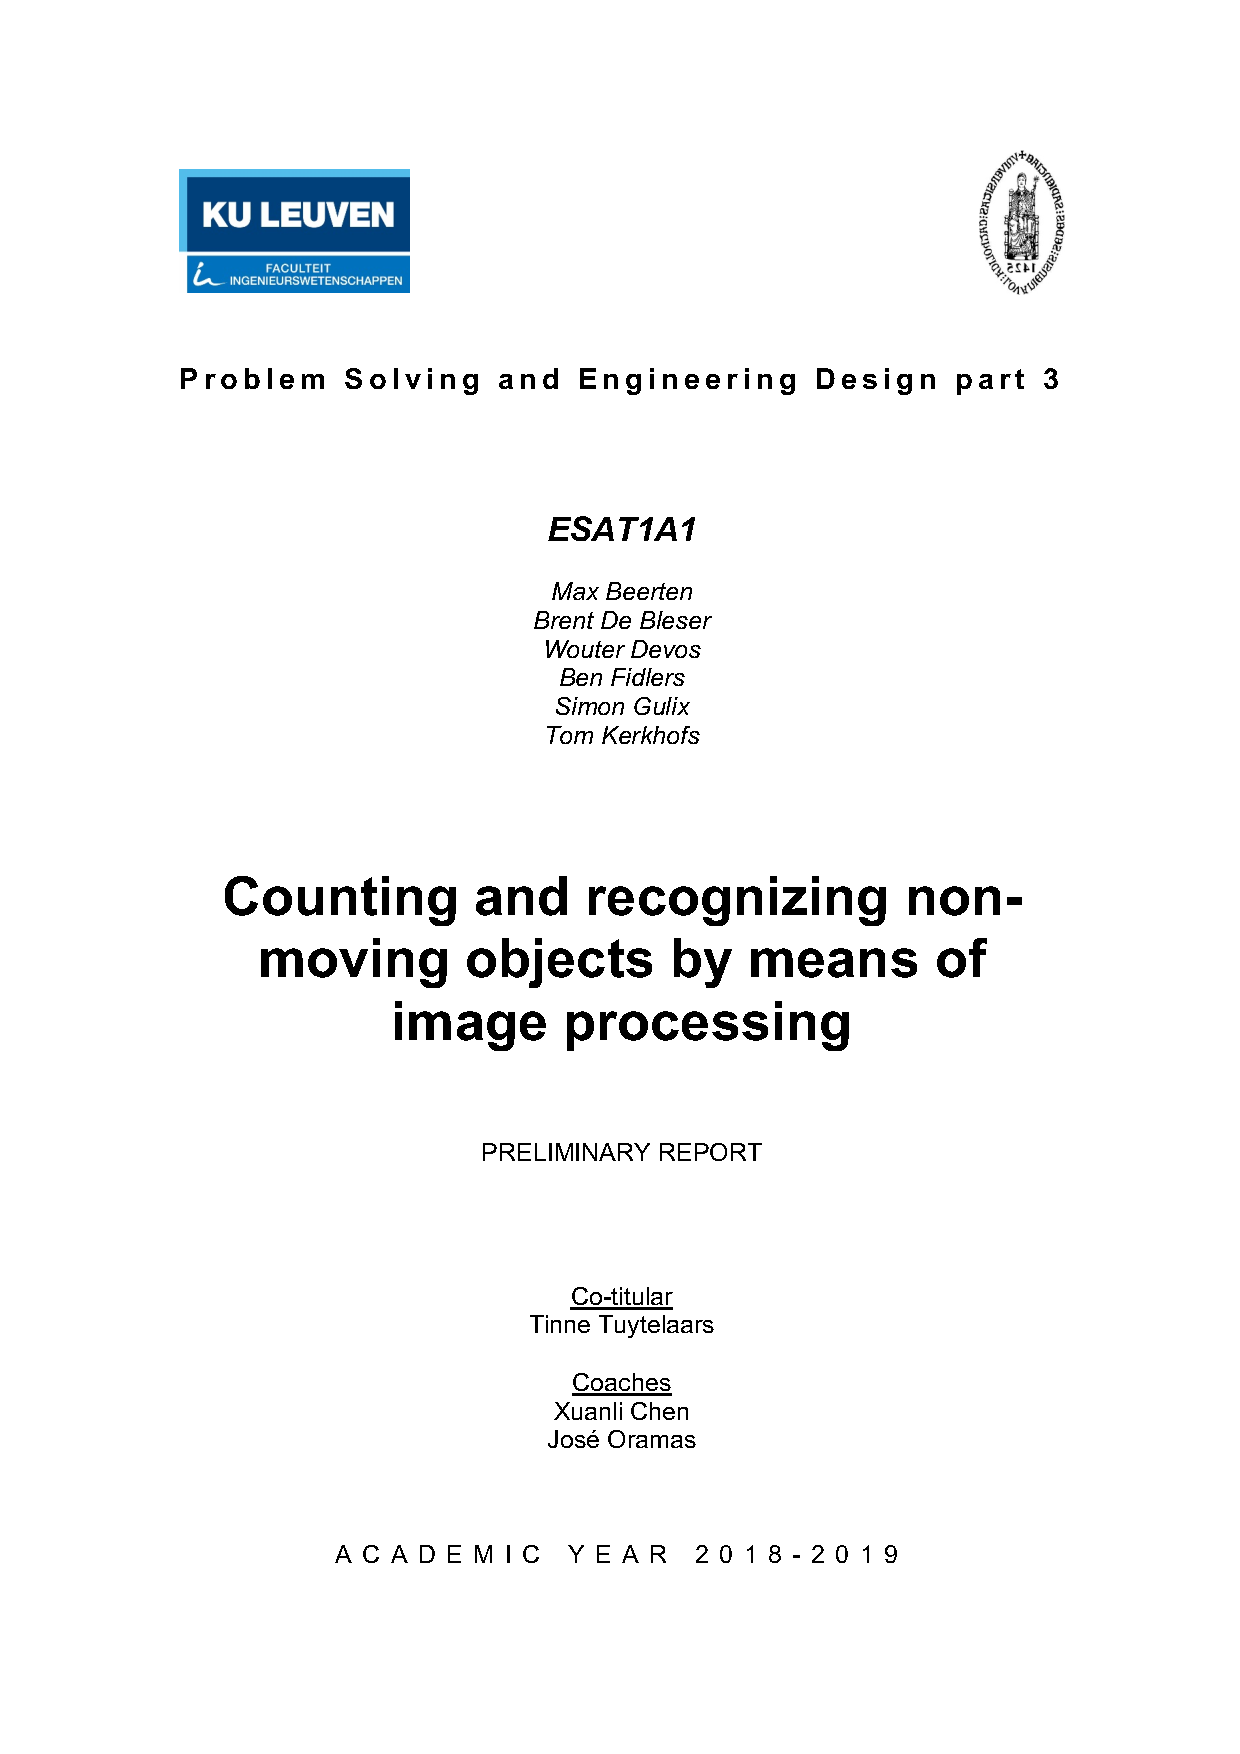
\includepdf[pages=-]{frontpage.pdf}

\section*{Abstract}
\thispagestyle{empty}

\newpage
\tableofcontents
\thispagestyle{empty}

\newpage
\listoftables
\thispagestyle{empty}

\newpage
\listoffigures
\thispagestyle{empty}

\newpage
\section{Introduction}
\pagenumbering{arabic}
Digital image processing has been a crucial part of the current digitalisation movement. From industrial machinery to customer amusement, the vision of computer-aided systems has become a given for most users. While image alteration and manipulation remain a core part of this image processing, nowadays other image related problems which used to be considered an important part of digital image processing are being solved by artificial intelligence. In this category sits the problem considered in this paper: feature extraction, the counting of objects in an image to be more exact. So why use 'traditional' methods to solve this problem? While being a great solution for many problems, artificial intelligence, as most general solutions certain cases are solved more efficiently by specific solutions. Such is the case with object counting, while deep learning algorithms need a big data set  as training material, standard image processing requires only the image itself.

\section{Problem Discription}

\hspace{\parindent} Given is a basket with a standard rectangular shape with fixed dimensions. The objective is to count every object in this basket. If possible, the objects can be outlined by the system.\\

\noindent The system used should be based on color and depth images.


\section{Design and implementation}
\subsection{Hardware}
\subsection{Software}
\subsubsection{Analysis colour image }

There are a lot of options when it comes to software and there exist many different algorithms for image processing. The diagram on FIG…XX… shows a couple of different methods. There is no ‘right-way’ to count objects in an image. Different methods have different advantages and disadvantages. The only things that appears in almost all algorithms are:
\begin{itemize}
\item Converting the RGB image to grayscale
\item Run filters over the image to remove noise
\end{itemize}
These things are also visible in the diagram.
\paragraph{Method 1}\mbox{}\\
This method is the most simple and easy to write. It starts with the grayscale image which has been filtered. Then it runs an thresholding-algorithm with a pre-defined threshold value over the image and the output is a binary image. That’s an image that only has 0’s and 1’s in his matrix.  It’s also possible to use an algorithm to search for the best threshold value.  After that there is a simple edge detection algorithm which makes the edges visible. 
Advantages: it’s an easy and fast algorithm.
Disadvantages: with a pre-defined threshold value it just classifies pixels based on colour. 
\paragraph{Method 2}\mbox{}\\
Method 2 is the reverse of method 1: it starts with an edge detection algorithm. But a different one than in method 1 and a bit more complicated. This algorithm gives back an greyscale image, not a binary image. After that is a threshold algorithm with a pre-defined threshold value and the edges are converted to a binary image. Because there is a lot of noise with this method, it's recommended to use a noise reduction algorithm. 
Advantages: it detects all kind of objects, not based on colour or shape.
Disadvantages: the boundary between different objects needs to be clear.
\paragraph{Method 3}\mbox{}\\
This method is different. It makes a compromise in functionality: it needs a picture of the background alone before it can detect objects. First it loads an background image, converts it to grayscale and runs some filters over the image. After that, the algorithm loops through the image pixel by pixel, checks if the pixel on the image is within a certain range of the same pixel on the background image. If the pixel is within that range, that pixel gets classified as background. The output is a binary image with only the objects.  
Advantages: it is better in detecting objects, not based on colour or shape.
Disadvantages: There needs to be an image of the empty background, and lightning conditions etc. can’t change.


\subsubsection{Analysis depth image}

\section{Implementation}
Throughout the project a lot of different approaches were tested and discarded. Right now 

\section{Budget management}

\section{Course Integration}

\section{Conclusion}

\section{List of references}

\section{Appendix}

\end{document}
